\chapter{Observations, Dark Matter, and the Cosmological Fit}

\lectureoverview{Observation acquires meaning only after it is connected to a cosmological model. We begin with the Friedmann equation and the three homogeneous spatial geometries, organize the present cosmic budget into radiation, matter, vacuum energy, and curvature, and reconstruct why an open universe once seemed unavoidable. Galaxy rotation curves then reveal the missing gravitating matter and lead to the dynamics of a cold, weakly interacting halo. Finally, redshift, brightness, and source counts turn a trial expansion history into observable curves. The old matter-plus-curvature model fails; a matter fraction near \(0.3\), a vacuum fraction near \(0.7\), and very small curvature give the lecture's successful fit.}

\section{Put the Observations Back Into the Equations}

Astronomical facts cannot be interpreted in isolation. We first need the equations that tell us which combinations of observations distinguish one universe from another. For a homogeneous and isotropic universe the starting point is Friedmann's equation,
\begin{equation}
\left(\frac{\dot a}{a}\right)^2
=
\frac{8\pi G}{3}\rho-\frac{k}{a^2}.
\label{eq:c06-friedmann}
\end{equation}
The quantity
\begin{equation}
H(t)=\frac{\dot a(t)}{a(t)}
\label{eq:c06-hubble}
\end{equation}
is the Hubble \emph{function}. Its present value \(H_0\) is conventionally called the Hubble constant, but \(H(t)\) is not constant over cosmic history. When astronomers quote a value in kilometers per second per megaparsec, they are quoting \(H_0\). \lecturetimestamp{00:00:09--00:02:03}

The normalized curvature label takes only three values,
\begin{equation}
k\in\{+1,0,-1\},
\end{equation}
corresponding respectively to spherical, flat, and hyperbolic spatial geometry. The common FRW metric may be written
\begin{equation}
ds^2=-dt^2+a(t)^2\left[dr^2+\xi(r)^2d\Omega_2^2\right],
\label{eq:c06-frw}
\end{equation}
where
\begin{equation}
\xi(r)=
\begin{cases}
\sin r, & k=+1,\\
r, & k=0,\\
\sinh r, & k=-1.
\end{cases}
\label{eq:c06-xi}
\end{equation}
This notation will do two jobs. It packages the three geometries into one metric, and later it gives the area of a sphere and therefore the number of sources in a radial shell. Thus a choice of \(k\) and an equation for \(a(t)\) is already a model with observational consequences. \lecturetimestamp{00:02:03--00:04:54}

\section{The Present Cosmic Budget}

The energy density has three principal components in the model under discussion: radiation, nonrelativistic matter, and vacuum energy. Including curvature on the same bookkeeping line gives
\begin{equation}
\frac{C_r}{a^4}
+\frac{C_m}{a^3}
+\Lambda
-\frac{k}{a^2}
=H^2.
\label{eq:c06-budget}
\end{equation}
Here \(\Lambda\) uses the normalization of the preceding lecture, \(\Lambda=(8\pi G/3)\rho_{\rm vac}\). Radiation dilutes as \(a^{-4}\), matter as \(a^{-3}\), vacuum energy does not dilute, and curvature scales as \(a^{-2}\). Curvature is not a material energy density, but placing it beside the other terms makes the present constraint transparent: the four contributions must add to \(H_0^2\). \lecturetimestamp{00:05:08--00:08:23}

Define their present fractions by
\begin{equation}
\Omega_r=\frac{C_r/a_0^4}{H_0^2},
\qquad
\Omega_m=\frac{C_m/a_0^3}{H_0^2},
\qquad
\Omega_\Lambda=\frac{\Lambda}{H_0^2},
\qquad
\Omega_k=\frac{-k/a_0^2}{H_0^2}.
\label{eq:c06-omegas}
\end{equation}
Then
\begin{equation}
\boxed{\Omega_r+\Omega_m+\Omega_\Lambda+\Omega_k=1.}
\label{eq:c06-sum-rule}
\end{equation}
The \(\Omega\)'s are ratios evaluated today, not time-independent constants. Also note the sign convention: \(k=-1\) gives a positive \(\Omega_k\). \lecturetimestamp{00:15:41--00:16:59}

\subsection{How the First Terms Are Measured}

Hubble obtained the local expansion rate by comparing recession redshift with distance. The redshift supplies a velocity at low \(z\); a calibrated brightness supplies a distance. His first numerical value was badly wrong, but the method was right. Because the galaxies were comparatively nearby, the measurement did not probe a large fraction of cosmic history and could treat \(H\) as its present value. \lecturetimestamp{00:08:25--00:10:00}

\begin{classroomqa}
\audiencequestion{How can brightness determine distance unless the intrinsic brightness is already known?}
\lecturerresponse{It cannot do so in one step. The cosmic distance ladder begins with parallax for nearby stars. Cepheid variables in that calibrated region reveal a period-luminosity relation and become standard candles for greater distances. Overlapping calibrations carry the ladder outward, and supernovae provide the best candles at the cosmological redshifts used later. Distance is therefore inferred from a chain of standards, not from an arbitrary assumption that every object shines equally. \lecturetimestamp{00:10:00--00:11:32}}
\end{classroomqa}

\begin{classroomqa}
\audiencequestion{Are \(C_r\) and \(C_m\) constants even though their densities change?}
\lecturerresponse{Yes. The coefficients remain fixed while the factors \(a^{-4}\) and \(a^{-3}\) carry the time dependence. Vacuum energy is constant, and curvature scales as \(a^{-2}\). These unequal powers are precisely why the fractional contributions change from one era to another. \lecturetimestamp{00:11:35--00:12:02}}
\end{classroomqa}

The radiation term can be measured locally from the photon background. Most of it is the cosmic microwave background, and its present energy density is tiny compared with the other important components. A sufficiently large averaging volume is required, but no long excursion down the past light cone is needed to establish that \(\Omega_r\) is negligible today. \lecturetimestamp{00:12:03--00:13:39}

Visible matter is estimated from galaxies, stellar populations, hydrogen, and interstellar gas. The methods are technical rather than conceptually obscure: determine the typical stellar and gas content, sum it over galaxies, and average over a large volume. The lecture quotes the old rough scale of one proton mass per cubic meter. This is much larger than the radiation density but still remarkably dilute. \lecturetimestamp{00:13:40--00:15:08}

\begin{classroomqa}
\audiencequestion{What about dark matter in this accounting?}
\lecturerresponse{It is coming, but first we deliberately reconstruct the older inference based on luminous matter alone. The historical order matters: it shows exactly which apparent conclusion dark matter corrected and which gap it did not close. \lecturetimestamp{00:15:08--00:15:40}}
\end{classroomqa}

\section{Why an Open Universe Once Seemed Necessary}

In the older picture, radiation was correctly judged negligible, vacuum energy was set to zero, and matter meant only the material visible through electromagnetic radiation. The resulting estimate was roughly
\begin{equation}
\Omega_r\simeq0,
\qquad
\Omega_\Lambda=0,
\qquad
\Omega_m^{\rm luminous}\sim\frac{1}{20}\text{--}\frac{1}{30}.
\end{equation}
The sum rule then appeared to force
\begin{equation}
\Omega_k\simeq1.
\end{equation}
Since a positive curvature contribution means \(-k/a_0^2>0\), this implied \(k=-1\): an open, negatively curved universe. These numbers are a reconstruction of the older argument, not a modern parameter estimate. \lecturetimestamp{00:17:00--00:19:50}

To interpret the curvature scale, return to the matter-dominated solution
\begin{equation}
a(t)\propto t^{2/3}.
\end{equation}
Differentiating and dividing by \(a\) gives
\begin{equation}
H(t)=\frac{\dot a}{a}=\frac{2}{3t}.
\label{eq:c06-matter-h}
\end{equation}
At the present age \(T\),
\begin{equation}
H_0\simeq\frac{2}{3T}.
\end{equation}
Thus the Hubble time is of the same order as the age of the universe. The radiation-dominated comparison,
\begin{equation}
a(t)\propto t^{1/2},
\qquad
H(t)=\frac{1}{2t},
\end{equation}
shows that this inverse-age relation is not peculiar to dust. \lecturetimestamp{00:19:50--00:24:50}

\begin{figure}[htbp]
\centering

\includegraphics[width=0.72\textwidth]{lecture_06_figure_02.png}
\caption{The matter-era board review. The visible writing contains \(a\sim t^{2/3}\) and \(\dot a/a=2/(3t)\); the lecturer obscures the remaining board, so no hidden equation is attributed to the frame.}
\label{fig:c06-age-board}
\lectureframe{00:24:41.615}
\end{figure}

\begin{classroomqa}
\audiencequestion{What units does the Hubble constant have, and where is the speed of light?}
\lecturerresponse{Since \(H\) relates velocity to distance, it has units of inverse time. It may be quoted in inverse seconds, inverse years, or the astronomers' equivalent kilometers per second per megaparsec. The relation \(H\sim1/T\) needs no extra \(c\). A factor of \(c\) appears only when the time \(T\) is translated into a length such as \(cT\). \lecturetimestamp{00:22:50--00:24:25}}
\end{classroomqa}

Hubble's original value of \(H_0\) was too large by roughly an order of magnitude, so the corresponding Hubble age was too short, of order a billion rather than ten billion years in the lecture's rounded comparison. Better calibration repaired the number without changing the logic that \(H_0^{-1}\) is a cosmic timescale. \lecturetimestamp{00:24:57--00:25:24}

The old curvature inference now reads
\begin{equation}
\frac{1}{a_0^2}\sim H_0^2\sim\frac{1}{T^2}.
\end{equation}
In units \(c=1\), the radius of curvature \(a_0\) was therefore thought to be of order the age \(T\); with ordinary units restored it was of order \(cT\). The lecture immediately withdraws this as a statement about the real universe. It is the conclusion one obtained several decades earlier after discarding the terms then believed negligible. \lecturetimestamp{00:25:51--00:27:41}

\begin{classroomqa}
\audiencequestion{If curvature was supposed to dominate today, why use the matter-dominated law \(a\propto t^{2/3}\)?}
\lecturerresponse{Because matter scales as \(a^{-3}\) while curvature scales only as \(a^{-2}\). At smaller \(a\), matter wins. Curvature could become important only late, so matter domination still described most of the elapsed history and kept \(H_0\) of order \(1/T\). A complete mixed solution would correct the numerical factor, not erase the timescale argument. \lecturetimestamp{00:49:20--00:50:17}}
\end{classroomqa}

\section{Dark Matter From Galactic Dynamics}

There are two operational ways to inventory matter. One is to count material that emits or absorbs light. The other is to infer mass from gravity. Oort found anomalous galactic dynamics in the early 1930s, and Zwicky found the analogous mass discrepancy in galaxy clusters. The evidence said that gravitating matter exceeded luminous matter. Ordinary charged matter radiates and collides; the missing component was known first by its gravitational action. \lecturetimestamp{00:27:45--00:29:50}

\begin{classroomqa}
\audiencequestion{Does luminous matter include diffuse gas and central black holes?}
\lecturerresponse{Diffuse gas is included insofar as its amount can be inferred from its electromagnetic behavior. A central supermassive black hole may be included in the known mass budget, but it is only a small fraction of a galaxy's total mass and is concentrated at the center. It cannot explain a discrepancy that persists far outside the luminous center. \lecturetimestamp{00:29:50--00:31:14}}
\end{classroomqa}

Consider a star moving approximately in a circular orbit of radius \(r\). If nearly all the mass \(M\) were concentrated near the galactic center, Newton's law would give
\begin{equation}
\frac{GM}{r^2}=\frac{v^2}{r},
\end{equation}
and hence
\begin{equation}
v^2=\frac{GM}{r},
\qquad
v(r)\propto r^{-1/2}.
\label{eq:c06-kepler}
\end{equation}
This is the Kepler falloff expected outside a central mass distribution. \lecturetimestamp{00:31:15--00:33:39}

\begin{figure}[htbp]
\centering

\includegraphics[width=0.78\textwidth]{lecture_06_figure_03.png}
\caption{The rotation-curve board at the transition from a central mass to an enclosed mass \(M(r)\). Only \(MG\), the fraction bar, the orbit sketch, and portions of the curve sketches are visible; equation~\eqref{eq:c06-kepler} comes from the spoken derivation.}
\label{fig:c06-rotation-board}
\lectureframe{00:34:53.642}
\end{figure}

\begin{figure}[htbp]
\centering
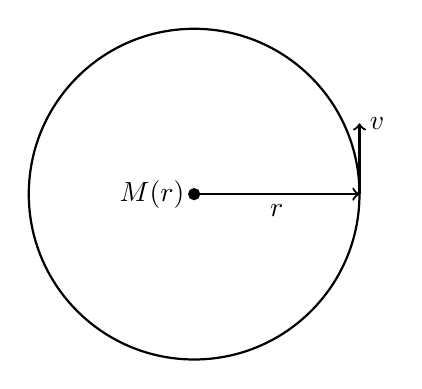
\begin{tikzpicture}[scale=1.0]
\filldraw (0,0) circle (2pt) node[left] {\(M(r)\)};
\draw[thick] (0,0) circle (2.1);
\draw[->,thick] (0,0)--(2.1,0) node[midway,below] {\(r\)};
\draw[->,thick] (2.1,0)--(2.1,0.9) node[right] {\(v\)};
\end{tikzpicture}
\caption{The circular-orbit construction used to infer enclosed mass from a measured rotation speed.}
\label{fig:c06-orbit-redraw}
\end{figure}

Observed galactic rotation curves do not fall in this way; over a substantial radial range they are approximately flat. Replace the fixed central mass by the enclosed mass \(M(r)\):
\begin{equation}
\frac{G M(r)}{r^2}=\frac{v(r)^2}{r}.
\end{equation}
If \(v(r)\) is nearly constant, then
\begin{equation}
\boxed{M(r)\propto r.}
\label{eq:c06-enclosed-mass}
\end{equation}
This refers to total mass inside radius \(r\), not to local density. The gravitating mass continues to grow well beyond the region where most starlight is concentrated. Motions perpendicular to galactic disks further indicate an approximately spherical distribution: a dark halo rather than a second thin disk. \lecturetimestamp{00:33:39--00:38:04}

\begin{classroomqa}
\audiencequestion{Is there a simple theory explaining why the rotation curve is so flat?}
\lecturerresponse{Not in this argument. Simulations of galaxy formation may make such profiles natural, but the lecture does not claim a short derivation. The secure statement is observational: nearly constant \(v\) implies approximately linear growth of enclosed mass. The neatness of that relation should not be mistaken for an elementary explanation of galaxy formation. \lecturetimestamp{00:35:58--00:37:33}}
\end{classroomqa}

\begin{classroomqa}
\audiencequestion{Are spiral arms simply material pinwheels produced by the varying angular speed \(v/r\)?}
\lecturerresponse{No simple pinwheel picture works. The visible pattern need not rotate with individual stars; density-wave or star-formation-wave descriptions are among the possibilities. The lecture uses this uncertainty to separate the robust halo inference from the more complicated problem of spiral structure. \lecturetimestamp{00:37:35--00:38:34; 00:47:03--00:47:47}}
\end{classroomqa}

The inferred dark mass is several times the luminous mass, quoted in the lecture only as an order-of-magnitude factor between roughly five and ten. The halo also extends beyond the visible galaxy. These are deliberately rough historical scales, not precise universal ratios for every system. \lecturetimestamp{00:38:34--00:39:50}

\section{What the Dark Matter Must Be Like}

Why does ordinary matter form bright compact disks while dark matter remains in a broad halo? Luminous matter can lose mechanical energy through electromagnetic collisions and radiation. Once it dissipates energy, gravity can pull it into a denser configuration. Dark matter appears electrically neutral and much more weakly interacting. Its particles orbit through the halo with little collision or radiation, so even over billions of years they do not lose enough energy to settle into the luminous disk. Gravitational radiation from galactic motion is far too weak to provide an alternative cooling mechanism. \lecturetimestamp{00:39:35--00:41:22}

\begin{classroomqa}
\audiencequestion{Does weakly interacting mean that dark matter obeys a different law of gravity?}
\lecturerresponse{No. It is assumed to gravitate in the ordinary way. Weak interaction here means the absence, or great suppression, of nongravitational collisions and electromagnetic radiation. Two dark particles still attract gravitationally; that attraction organizes a halo but does not efficiently dissipate orbital energy. \lecturetimestamp{00:42:36--00:43:35}}
\end{classroomqa}

\begin{classroomqa}
\audiencequestion{What observations show that this is not only a peculiarity of one galactic rotation curve?}
\lecturerresponse{The evidence appears on several scales: stellar motion within galaxies, motion perpendicular to galactic planes, interactions between galaxies, and the dynamics of whole galaxy clusters. Oort's and Zwicky's examples were different manifestations of the same missing-gravity problem. \lecturetimestamp{00:42:00--00:42:36}}
\end{classroomqa}

\begin{classroomqa}
\audiencequestion{Should dark matter congregate around black holes and galactic centers?}
\lecturerresponse{It does become denser toward a gravitational center, but the historical sequence is likely the reverse of a halo forming around a pre-existing black hole. Dark halos formed large gravitational wells; baryonic matter then fell into them and formed galaxies, stars, and central black holes. The black hole is a small part of the mass. Searches for annihilation products nevertheless look toward the galactic center because the dark-matter density is expected to be higher there. \lecturetimestamp{00:43:36--00:45:43}}
\end{classroomqa}

\begin{classroomqa}
\audiencequestion{Is dark matter a gas, dust, compact clumps, or isolated particles? Could some be trapped near the Sun?}
\lecturerresponse{Its microscopic nature is unknown, but ordinary dust is bound by electromagnetic forces, exactly the sort of interactions dark matter seems to lack. The default particle picture is therefore a dilute population of individual particles. Some may be gravitationally concentrated near the Sun, yet their density is far too small to compete with solar gravity or disturb planetary dynamics. \lecturetimestamp{00:45:43--00:47:02; 00:58:41--00:59:29}}
\end{classroomqa}

The second central requirement is that the dark matter cluster. A hot population with relativistic random speeds resists gravitational aggregation; a cold population can fall into potential wells. Ordinary light neutrinos would have behaved as hot dark matter and do not provide the required primary galactic component. In this context \emph{cold} means nonrelativistic in the local cosmological frame, not literally at laboratory zero temperature. \lecturetimestamp{00:47:47--00:49:20}

\begin{classroomqa}
\audiencequestion{Does the requirement of cold clustering impose a dark-matter mass range?}
\lecturerresponse{It depends on quantum statistics and production history. Very light fermions cannot all occupy one slow state and are strongly constrained. Very light bosons can occupy a coherent Bose-condensed state; axions provide the lecture's example. Alternatively, heavier weakly interacting particles can be cold without condensation. Thus there is no model-independent single mass bound supplied by this argument. \lecturetimestamp{00:53:17--00:54:52; 00:56:42--00:58:05}}
\end{classroomqa}

\begin{classroomqa}
\audiencequestion{Should accelerators already have found the particles?}
\lecturerresponse{Only under additional assumptions. If the particles have roughly weak-interaction cross sections and masses within accelerator reach, collider production may be possible. The lecture's expectation of imminent information was explicitly speculative and historically dated. A particle could instead be too heavy or interact too feebly for the available experiments. \lecturetimestamp{00:54:52--00:55:54}}
\end{classroomqa}

\begin{classroomqa}
\audiencequestion{Could dark matter merely live in an unseen extra dimension?}
\lecturerresponse{No such mechanism is needed in the discussion. Dark matter is already observed gravitationally and may simply consist of unusual particles with almost no interaction with ordinary material. Calling an interaction weak is not the same as placing the particles outside observable spacetime. \lecturetimestamp{00:55:54--00:56:41}}
\end{classroomqa}

Modifying gravity rather than adding unseen matter is a logical alternative. The lecture judges that no comparably simple modification then explained the evidence across all relevant scales while retaining the successful solar-system laws. The particle interpretation is therefore preferred, but its microphysics remains unknown. \lecturetimestamp{00:58:08--00:59:29}

\section{Dark Matter Does Not Close the Old Budget}

Dark matter enlarges the matter contribution by a factor of several, but the old discrepancy between luminous matter and \(H_0^2\) was of order twenty-five. It therefore narrows the gap without making
\begin{equation}
\frac{C_m}{a_0^3}=H_0^2.
\end{equation}
Within the old no-\(\Lambda\) picture, a positive curvature-budget term and hence \(k<0\) were still required. There was nothing logically inconsistent about such an open model; the point is that dark matter alone did not select the modern answer. \lecturetimestamp{00:51:51--00:53:17}

\begin{classroomqa}
\audiencequestion{What did cosmologists actually think about curvature before the modern fit?}
\lecturerresponse{The evidence was confusing and prior preference for a closed, bounded universe sometimes pulled against the matter budget. Once the old assumptions were combined consistently, negative curvature was the natural inference. That historical consensus was still provisional because neither dark matter nor vacuum energy was securely incorporated in the way they are today. \lecturetimestamp{00:50:17--00:51:50}}
\end{classroomqa}

We must therefore test the candidate model rather than infer its truth from one budget line. A model consists of a curvature choice \(k\) and an expansion history \(a(t)\), equivalently a set of material equations of state and present parameters from which \(a(t)\) is computed. The old candidate is matter plus negative curvature with negligible radiation and no cosmological constant. \lecturetimestamp{00:59:34--01:01:00}

\section{Turn Geometry Into Observables}

\subsection{Source Counts and Brightness in a Frozen Geometry}

Temporarily ignore cosmic evolution. In a homogeneous universe the number of sources in a comoving shell is proportional to its area:
\begin{equation}
dN\propto \xi(r)^2\,dr.
\label{eq:c06-shell-count}
\end{equation}
Thus
\begin{equation}
dN\propto
\begin{cases}
\sin^2r\,dr, & k=+1,\\
r^2\,dr, & k=0,\\
\sinh^2r\,dr, & k=-1.
\end{cases}
\end{equation}
At large \(r\), the negatively curved case grows as \(\sinh^2r\sim e^{2r}\), far faster than the flat \(r^2\) law. Negative curvature therefore predicts an anomalously rapid increase in the number of sources with distance. \lecturetimestamp{01:01:29--01:04:10}

The same area controls received flux. In flat static space a standard source gives
\begin{equation}
F\propto\frac{1}{r^2}.
\end{equation}
In hyperbolic space the sphere over which radiation spreads grows faster, so the flux falls faster. The lecture sometimes calls this observed quantity luminosity; here \(F\) denotes brightness or flux, while intrinsic luminosity belongs to the source. Counts and brightness together can therefore distinguish spatial geometries. \lecturetimestamp{01:04:12--01:06:22}

\subsection{Redshift and the Past Light Cone}

The real universe evolves, and looking outward means looking backward in time. Light emitted at \(t_{\rm em}\) is stretched while the scale factor grows from \(a(t_{\rm em})\) to \(a_0\):
\begin{equation}
1+z
=\frac{\lambda_{\rm obs}}{\lambda_{\rm em}}
=\frac{a_0}{a(t_{\rm em})}.
\label{eq:c06-redshift}
\end{equation}
Equivalently,
\begin{equation}
z=\frac{\lambda_{\rm obs}}{\lambda_{\rm em}}-1.
\end{equation}
Different points along our past light cone correspond simultaneously to different comoving radii and different emission times. Expansion changes the wavelength; Doppler and gravitational shifts are other physical mechanisms, but cosmological expansion is the effect at issue here. \lecturetimestamp{01:06:48--01:11:38}

\begin{classroomqa}
\audiencequestion{Why does the definition of \(z\) contain the minus one?}
\lecturerresponse{It is a historical convention chosen so that an unshifted source has \(z=0\). The physically direct stretch factor is \(1+z=\lambda_{\rm obs}/\lambda_{\rm em}\). \lecturetimestamp{01:10:11--01:10:45}}
\end{classroomqa}

Radial light has \(d\Omega_2=0\) and follows \(ds^2=0\). Equation~\eqref{eq:c06-frw} therefore gives
\begin{equation}
dt^2=a(t)^2dr^2.
\end{equation}
For an incoming ray followed backward from us,
\begin{equation}
dt=-a(t)\,dr,
\qquad
\frac{dr}{dt}=-\frac{1}{a(t)}.
\label{eq:c06-null-ray}
\end{equation}
The minus sign says that larger comoving radius lies at earlier time along the ray. Once \(a(t)\) is known, this equation determines \(r(t)\). \lecturetimestamp{01:11:52--01:14:06}

\subsection{Number Per Unit Redshift}

An observer can count standard sources in a redshift bin \(z\) to \(z+dz\). Begin with equation~\eqref{eq:c06-shell-count} and differentiate equation~\eqref{eq:c06-redshift} along the past light ray:
\begin{equation}
dz=-\frac{a_0}{a^2}\,da
=-\frac{a_0}{a^2}\dot a\,dt.
\end{equation}
Using \(dt=-a\,dr\),
\begin{equation}
dz=\frac{a_0}{a}\dot a\,dr
=(1+z)\dot a\,dr.
\end{equation}
Hence
\begin{equation}
dr=\frac{dz}{(1+z)\dot a},
\end{equation}
and, for a fixed comoving source density,
\begin{equation}
\boxed{
\frac{dN}{dz}
\propto
\frac{\xi(r)^2}{(1+z)\dot a}
}.
\label{eq:c06-dndz}
\end{equation}
The live derivation checks signs and factors more than once; equations~\eqref{eq:c06-null-ray} and \eqref{eq:c06-redshift} fix the result unambiguously. \lecturetimestamp{01:14:19--01:20:21}

\begin{figure}[htbp]
\centering

\includegraphics[width=0.84\textwidth]{lecture_06_figure_05.png}
\caption{The board relation between \(dN/dz\) and the model functions. The left side and \(a\sim t^{2/3}\), \(\dot a\), and \(r(t)\) on the right are visible, while the lecturer obscures part of the denominator; equation~\eqref{eq:c06-dndz} is established independently above.}
\label{fig:c06-dndz-board}
\lectureframe{01:22:24.114}
\end{figure}

There is nothing further to evaluate until a model is chosen. A specified \(a(t)\) determines \(\dot a(t)\), equation~\eqref{eq:c06-null-ray} determines \(r(t)\), and equation~\eqref{eq:c06-redshift} lets every quantity be expressed in terms of \(z\). Different equations of state produce different functions \(dN/dz\) and \(F(z)\). This is exactly what makes the observations discriminating. \lecturetimestamp{01:20:21--01:23:10}

\section{From Trial Parameters to the Best Fit}

The procedure is direct:
\begin{equation}
(\Omega_r,\Omega_m,\Omega_\Lambda,\Omega_k)
\longrightarrow
a(t)
\longrightarrow
\left\{F(z),\frac{dN}{dz}\right\}.
\label{eq:c06-fit-pipeline}
\end{equation}
Choose present parameters, solve Friedmann's equation, propagate radial light, compute brightness and counts versus redshift, and compare the curves with data. A failed comparison rejects the parameter set. Together, the two observables constrain both the expansion history and the spatial geometry. \lecturetimestamp{01:23:10--01:24:21}

\begin{figure}[htbp]
\centering

\includegraphics[width=0.84\textwidth]{lecture_06_figure_06.png}
\caption{The old matter-plus-curvature model on the upper board and the flat and hyperbolic shell factors \(r^2dr\) and \(e^{2r}dr\) on the lower board. Parts of the Friedmann equation are covered, so the frame is supporting evidence rather than an equation source.}
\label{fig:c06-old-model-board}
\lectureframe{01:24:27.863}
\end{figure}

The old model,
\begin{equation}
H^2=\frac{C_m}{a^3}-\frac{k}{a^2},
\qquad k=-1,
\end{equation}
fails both the brightness-redshift relation and the source-count test. Supernovae provide the most useful standard candles in the relevant redshift range. The lecture's successful parameter set is
\begin{equation}
\boxed{
\Omega_r\simeq0,\qquad
\Omega_m\simeq0.3,\qquad
\Omega_\Lambda\simeq0.7,\qquad
\Omega_k\simeq0
}.
\label{eq:c06-best-fit}
\end{equation}
Matter here includes luminous and dark matter. These values report the lecture-era fit; the durable lesson is the fitting method and the need for a dominant nondiluting component, not the last printed decimal. \lecturetimestamp{01:24:22--01:27:07}

\subsection{Questions About What Is Measured and What Is Fitted}

\begin{classroomqa}
\audiencequestion{Was \(\Lambda\) already assumed while the old open-universe model was being discussed?}
\lecturerresponse{No. The first part deliberately reconstructed the older model with \(\Lambda=0\). The values in equation~\eqref{eq:c06-best-fit} describe the later, modern fit. The old candidate was not amended silently; it was tested against \(F(z)\) and \(dN/dz\) and failed. \lecturetimestamp{01:26:45--01:27:07}}
\end{classroomqa}

\begin{classroomqa}
\audiencequestion{How is \(\Omega_\Lambda\) obtained if vacuum energy is not measured directly like local matter?}
\lecturerresponse{Begin with trial parameter sets. Each set defines a Friedmann solution and therefore predicted functions \(F(z)\) and \(dN/dz\). Compare those predictions with observations, discard poor fits, and retain the best region of parameter space. The number \(0.7\) is an inference from the fit, not a direct reading from a vacuum-energy meter. \lecturetimestamp{01:27:08--01:29:59; 01:31:57--01:33:40}}
\end{classroomqa}

\begin{classroomqa}
\audiencequestion{Where does the present scale \(a_0\) come from?}
\lecturerresponse{The normalization of \(a\) is partly conventional, but a completed model tied to \(H_0\) supplies the present physical curvature scale when \(k\ne0\). Once the model fits the redshift observables, its function \(a(t)\) identifies the present point and the corresponding scale. \lecturetimestamp{01:29:59--01:30:42}}
\end{classroomqa}

\begin{classroomqa}
\audiencequestion{Does looking billions of years into the past distort a fit based on today's parameters?}
\lecturerresponse{The lookback is not a distortion; it is the signal. Today's parameters are inserted into Friedmann's equation, which evolves them into a complete \(a(t)\). The predicted light cone already includes the fact that matter was more important at smaller \(a\), and sufficiently far back radiation dominates. A model that ignored this evolution would fail the data. \lecturetimestamp{01:30:43--01:31:55}}
\end{classroomqa}

\begin{classroomqa}
\audiencequestion{Which present quantities are measured comparatively directly?}
\lecturerresponse{The radiation density is measured and negligible today. The Hubble rate is measured from the distance-redshift relation. The total matter density is inferred gravitationally, including luminous and dark matter, and divided by the critical scale \(3H_0^2/(8\pi G)\) to obtain \(\Omega_m\). The remaining late-time freedom lies mainly in vacuum energy and curvature. \lecturetimestamp{01:33:40--01:35:32}}
\end{classroomqa}

\begin{classroomqa}
\audiencequestion{If both \(\Omega_\Lambda\) and \(\Omega_k\) are unknown, why is there only one independent late-time trial parameter after \(\Omega_m\) is fixed?}
\lecturerresponse{Because equation~\eqref{eq:c06-sum-rule} imposes one constraint. With \(\Omega_r\) negligible and \(\Omega_m\) measured, choosing a trial \(\Omega_\Lambda\) fixes the leftover \(\Omega_k=1-\Omega_m-\Omega_\Lambda\). One may equally parametrize the same one-dimensional family by curvature. For example, \(\Omega_\Lambda=0.4\) and \(\Omega_k=0.3\) is a valid trial when \(\Omega_m=0.3\); it is rejected only because its predicted curves fit poorly, not because the sum rule forbids it. \lecturetimestamp{01:35:33--01:39:09}}
\end{classroomqa}

\begin{classroomqa}
\audiencequestion{How can \(k\) be only \(+1,0,-1\) while \(\Omega_k\) varies continuously, and are the dimensions correct?}
\lecturerresponse{The discrete \(k\) records only the sign and normalized geometry. The continuous curvature radius is carried by \(a_0\), so \(-k/(a_0^2H_0^2)\) can take a continuum of values. In units \(c=1\), inverse length and inverse time have the same dimensions; restoring conventional units supplies the required powers of \(c\). \lecturetimestamp{01:39:10--01:40:07}}
\end{classroomqa}

\begin{classroomqa}
\audiencequestion{Does the count method assume homogeneity and isotropy, even though galaxy populations evolve?}
\lecturerresponse{It assumes spatial homogeneity and isotropy on sufficiently large slices, and those symmetries can be tested by comparing different directions at the same redshift. Source evolution is a separate issue: populations at different epochs need not be identical, so practical analyses model selection and evolution rather than pretending the number density is eternally fixed. The simple derivation isolates the geometric factor before those refinements are added. \lecturetimestamp{01:40:08--01:41:08}}
\end{classroomqa}

\section{The Density Fractions Evolve}

Equation~\eqref{eq:c06-budget} holds at every time, but the \(\Omega\)'s in equation~\eqref{eq:c06-omegas} were defined at the present time. Their time-dependent analogues change because the four terms have different powers of \(a\). Far in the past,
\begin{equation}
\Omega_r(t)\longrightarrow1.
\end{equation}
As radiation dilutes faster, matter rises toward dominance. Later, matter itself dilutes while \(\Lambda\) remains fixed, so in the far future,
\begin{equation}
\Omega_\Lambda(t)\longrightarrow1.
\end{equation}
The matter fraction therefore begins small, becomes close to unity during the matter era, and falls again after vacuum energy takes over. Curvature, if nonzero, eventually loses to a positive constant \(\Lambda\) as well. \lecturetimestamp{01:41:08--01:45:39}

\begin{classroomqa}
\audiencequestion{Does a small present curvature fraction mean the universe becomes flatter as it expands?}
\lecturerresponse{Its physical curvature scale grows with \(a\), and relative to a positive cosmological constant the curvature contribution \(a^{-2}\) becomes ever less important. This is the sense of the phrase \emph{big is flat}. It does not change the discrete topology label \(k\); it says local curvature and the fractional dynamical importance of curvature decrease. \lecturetimestamp{01:47:13--01:47:42}}
\end{classroomqa}

\begin{classroomqa}
\audiencequestion{Did the fitted model show unexplained systematic residuals, and how precise was the claim?}
\lecturerresponse{The lecture reports no known systematic failure of the framework at that level and describes it as precision cosmology at roughly the percent scale, not at a tenth or hundredth of a percent. That statement is historical and should not be converted into a timeless current error bar. \lecturetimestamp{01:45:40--01:46:19}}
\end{classroomqa}

\begin{classroomqa}
\audiencequestion{Can spatial curvature be tested by direct triangulation rather than only by supernova brightness and counts?}
\lecturerresponse{Yes. The angular pattern of the cosmic microwave background supplies a standard physical scale and therefore a large cosmic triangle. Supernova data alone did not provide the lecture's full percent-level curvature statement; combining them with microwave-background geometry sharpened the test. This is the subject of the next lecture. \lecturetimestamp{01:46:19--01:47:12}}
\end{classroomqa}

\section{What to Carry Forward}

The central lesson is not a catalogue of four numbers. It is a method. A cosmological parameter set produces \(a(t)\); the metric then predicts the propagation of light, source brightness, and source counts. Agreement tests both the chosen parameters and the Friedmann framework that connects them. There is no reason an arbitrary set must fit.

The old luminous-matter, negative-curvature model failed. Dark matter repaired the gravitating matter inventory but did not by itself close the old Friedmann budget. The successful lecture-era fit required approximately
\begin{equation}
\Omega_m\simeq0.3,
\qquad
\Omega_\Lambda\simeq0.7,
\qquad
\Omega_k\simeq0,
\end{equation}
and its curvature precision depended importantly on the microwave background. The model is credible because several independent observations pass through one dynamical theory and meet in the same region of parameter space. \lecturetimestamp{01:47:42--01:48:35}
